%!TEX options = -shell-escape

\documentclass[a4paper]{article} 
\usepackage{amsmath}
\usepackage{enumitem}
\usepackage{commath2, commath2-additions}
\usepackage[parfill]{parskip}

% required load order: (float - fix \listoflistings) - hyperref - minted
\usepackage[section]{placeins}
\usepackage{hyperref}

%% minted %%
\usepackage[newfloat]{minted}
\usepackage{xcolor}
\usemintedstyle{colorful}
\definecolor{codebg}{rgb}{0.95,0.95,0.95}
% \definecolor{codehl}{HTML}{FDF6E3}
\definecolor{codehl}{rgb}{0.90,0.90,0.90}
\newminted[cppcode]{cpp}{ % use \begin{cppcode}
    mathescape,
    bgcolor = codebg,
    fontsize = \footnotesize,
    breaklines,
}
\newminted[plaincppcode]{cpp}{ % use \begin{cppplaincode}
    mathescape,
    fontsize = \footnotesize,
    breaklines,
}
\newmintinline[cppinline]{cpp}{breaklines} % use \cppinline
\newmint[cppmint]{cpp}{breaklines}
\newmintedfile[cppfile]{cpp}{ % use \cppfile[<options>]{<filename>}
    mathescape,
    bgcolor = codebg,
    fontsize = \footnotesize,
    breaklines,
}
\usepackage[capitalise]{cleveref}
\usepackage{graphicx}
\graphicspath{{../figs/}}
\usepackage{subcaption}
\usepackage{todonotes}
\usepackage[font=small,labelfont=bf,width=0.9\textwidth]{caption}

%% commands %%
\newcommand{\cpp}{\texttt{C++}}
\newcommand{\python}{\texttt{Python}}
\newcommand{\cppeleven}{\texttt{C++11}}

%% "task x.x enumerate list" %%
% \newlist{tasks}{enumerate}{1}
% \setenumerate[tasks]{wide, labelwidth=!, labelindent=0pt, listparindent=0pt, label=\textbf{Task \thesection.\arabic*}}

\setlength{\belowcaptionskip}{0.0pt} % 0.0pt
\setlength{\abovecaptionskip}{8.0pt} % 10.0pt

\title{FY8904 Assignment 1}
\date{Spring 2019}
\author{Filip Sund}

\begin{document}
\maketitle

\section*{Notes on code}
Most of my code is \cpp\, and make extensive use of the Armadillo \cpp\ matrix library\footnote{See \url{http://arma.sourceforge.net/docs.html} for documentation.}. 

\begin{itemize}
    \item \cppinline{Mat} is the base matrix type in Armadillo
    \item \cppinline{Col} is the base column vector type in Armadillo
    \item \mintinline{c++}{mat} is typedef for \mintinline{c++}{Mat<double>}
    \item \mintinline{c++}{vec} is typedef for \mintinline{c++}{Col<double>}
    \item \mintinline{c++}{umat} is typedef for \mintinline{c++}{Mat<uword>}
    \item \mintinline{c++}{imat} is typedef for \mintinline{c++}{Mat<sword>}
    \item \mintinline{c++}{uvec} is typedef for \mintinline{c++}{Col<uword>}
    \item \mintinline{c++}{ivec} is typedef for \mintinline{c++}{Col<sword>}
    \item \mintinline{c++}{uword} is typedef for an \emph{unsigned} integer type
    \item \mintinline{c++}{sword} is typedef for an \emph{signed} integer type
\end{itemize}
The minimum width for \mintinline{c++}{uword} and \mintinline{c++}{sword} is 64 bits on 64-bit platforms when using \cppeleven\ and newer standards, and 32 bits when using older \cpp\ standards.

\setcounter{section}{1}
\section{The lattice}
\subsection*{Task 2.1}
See \cref{lst:makebonds} for a \cpp\ code snippet that, given a number of sites $N = m\times n$ returns a list of pairs of nodes connected by a bond in a square lattice of size $(m, n)$ and periodic boundary conditions. 

\begin{listing}[h!]
\cppfile[firstline=28, lastline=52]{../cpp_bond_percolation/src/lattices.hpp}%
\caption{%
    A \cpp\ code snippet for generating the bonds in a rectangular lattice, using periodic boundary conditions.%
    \label{lst:makebonds}%
}
\end{listing}
\FloatBarrier

I have omitted writing to a file, since I will be calling this code on the fly when the program runs. The code runs fast enough that there's no reason to generate the bonds/lattice ahead of time. Saving to a file is trivially achieved via for example
\mintinline{c++}{bonds.save("bonds.csv", arma::csv_ascii)}.

Example output for a square lattice of size $(3, 3)$
\begin{cppcode}
0  0  1  1  2  2  3  3  4  4  5  5  6  6  7  7  8  8
1  3  2  4  0  5  4  6  5  7  3  8  7  0  8  1  6  2
\end{cppcode}

\subsection*{Task 2.2}

In \cref{fig:lattices} the three different lattices are illustrated, with a simplified ``unit cell'' indicated in blue. By counting the number of bonds in each unit cell (including $1/2$ bonds) we can figure out the number of bonds in a lattice of size $N$.
\begin{figure}[htb!]
    \centering
    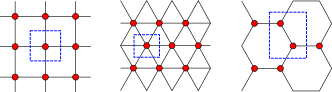
\includegraphics{lattice.pdf}
    \caption{Illustrations of different lattices.\label{fig:lattices}, with simplified unit cells drawn in blue.}
\end{figure}

In a \emph{square} lattice we have $4\times 1/2$ bonds in the unit cell, so for a lattice of size $N = L*L$ we have $2N$ bonds.

In a \emph{trianglular} lattice we have $6\times 1/2$ bonds in the unit cell, for a total of $3N$ bonds in a lattice of size $N$.

In a \emph{honeycomb} lattice we have $1 + 3\times 1/2$ bonds and 2 nodes in the unit cell, for a total of $3N/2$ bonds in a lattice of size $N$.

\subsection*{Task 2.3}
See \cref{lst:maketriangularbonds,lst:makehoneycombbonds} for code that generates the bonds for triangular and honeycomb lattices. The numbering schemes used are illustrated in \cref{fig:otherlattices}.

\begin{figure}[htb!]
    \centering
    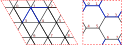
\includegraphics[width=0.9\textwidth]{both_lattices.pdf}%
    \caption{Illustrations a triangular lattice (left) and a honeycomb lattice (right) with periodic boundary conditions and the numbering scheme for the nodes/sites used in this report. The red dashed boundary illustrate the periodic boundaries, and the blue lines indicate the bonds that are added to the list of bonds at each step in \cref{lst:maketriangularbonds,lst:makehoneycombbonds}. \label{fig:otherlattices}}
\end{figure}

\begin{listing}[h!]
\cppfile[firstline=54, lastline=83]{../cpp_bond_percolation/src/lattices.hpp}%
\caption{%
    Program that generates bonds for a triangular lattice with periodic boundary conditions. %
    \label{lst:maketriangularbonds}%
}
\end{listing}

\begin{listing}[h!]
\cppfile[firstline=85, lastline=86]{../cpp_bond_percolation/src/lattices.hpp}%
\caption{%
    Program that generates bonds for a honeycomb lattice with periodic boundary conditions. %
    \label{lst:makehoneycombbonds}%
}
\end{listing}

Example output for the lattices illustrated in \cref{fig:otherlattices} (a 3x4 triangular lattice and a 2x4 honeycomb lattice):
\begin{minted}{cpp}
// 3x3 triangular lattice
0  0  0  1  1  1  2  2  2  3  3  3  4  4  4  5  5  5  6  6  6  7  7  7
1  4  7  2  5  4  3  6  5  0  7  6  5  0  3  6  1  0  7  2  1  4  3  2

// 2x4 honeycomb lattice
0  0  1  1  2  3  4  4  5  5  6  7
7  1  6  2  3  0  3  5  2  6  7  4
\end{minted}

\section{Percolating the system}
\subsection*{Task 3.1}
Since I generate lattices on the fly instead of saving to files, I have omitted code for saving to and reading nodes/bonds from files. But using the Armadillo \cpp\ library, reading a matrix from a CSV-file is done using
\begin{minted}{cpp}
umat bonds;
bonds.load("bonds.csv", arma::csv_ascii);
\end{minted}

NB! Since the default \cppinline!vec! type in Armadillo is a column vector, I store the bonds in a matrix of size $(2, M)$ instead of $(M, 2)$.

\subsection*{Task 3.2}
I use a 32-bit Mersenne Twister from the \cpp-header \mintinline{cpp}!random!. This can be initialized to any seed via

\mint{cpp}!static std::mt19937 rng(seed);!

A uniform integer distribution which produces integer values in the (closed) interval $\left[a, b\right]$ is created as follows

\mint{cpp}!std::uniform_int_distribution<uword> uniform(a, b);!

And random numbers are generated using

\begin{minted}{cpp}
for (uword i = 0; i < 10; i++)
{
    cout << uniform(rng) << endl;
}
\end{minted}

This will generate the same 10 random numbers if the seed is the same. The RNG \mintinline{cpp}!rng! can be seeded using a random number as follows
\begin{minted}{cpp}
static std::random_device rd;
static std::mt19937 rng(rd());
\end{minted}
(\mintinline{cpp}!std::random_device! is platform specific, so if a non-deterministic source of randomness is not available this might not produce non-deterministic seeds. In our case this is not an issue, but check your implementations documentation to see what the case is for any work that requires non-deterministic seeds.)

\subsection*{Task 3.3}
Code for shuffling the list of bonds can be seen in \cref{lst:shufflebonds}. This code is not very optimized, since we create a new random distribution every step of the loop, but it does not appear to be any kind of bottleneck compared to the rest of the program.
\begin{listing}[h!]
\cppfile[firstline=17, lastline=26]{../cpp_bond_percolation/src/lattices.hpp}%
\caption{%
    A \cpp\ code snippet for shuffling the columns in a Armadillo matrix, utilizing the \cppinline{.swap_cols} function from Armadillo. Bonds are stored in a $(2, M)$ matrix.%
    \label{lst:shufflebonds}%
}
\end{listing}
\FloatBarrier

\subsection*{Task 3.4}
The status of each node is kept in a \cppinline!ivec! (signed integer vector), and is initialized to $-1$ using
\cppmint!imat sites = zeros<ivec>(m*n) - 1!

\subsection*{Task 3.5}
I have implemented the root finding function as a member of a class \cppinline{Sites}, defined as \cppinline{uword findRoot(const uword site)}. The implementation can be seen in \cref{lst:findroot}.
\begin{listing}[h!]
\cppfile[firstline=92, lastline=111]{../cpp_bond_percolation/src/sites.cpp}%
\caption{%
    Member function of the class \cppinline{Sites} that finds the root node of a site \cppinline{site}. \cppinline{m_sites} is a member variable of \cppinline{Sites} with type \cppinline{ivec}.%
    \label{lst:findroot}%
}
\end{listing}
\FloatBarrier

\subsection*{Task 3.6}
The function for activating a bond (a member of the class \cppinline{Sites}) is given in \cref{lst:activate,lst:mergeclusters}.
\begin{listing}[h!]
\cppfile[firstline=18, lastline=33]{../cpp_bond_percolation/src/sites.cpp}%
\caption{%
    Member function of the class \cppinline{Sites} that activates a bond \cppinline{bond}. See \cref{lst:mergeclusters} for the implementation of the function \cppinline{mergeClusters}.%
    \label{lst:activate}%
}
\end{listing}

\begin{listing}[h!]
\begin{cppcode}
void Sites::mergeClusters(const uword root1, const uword root2)
{
    uword larger = root1;
    uword smaller = root2;
    if (m_sites(root2) < m_sites(root1)) // if root2 cluster is larger
    {
        larger = root2;
        smaller = root1;
    }

    // add size of smaller cluster to larger cluster
    m_sites(larger) += m_sites(smaller);

    // point root node of smaller cluster root node of larger cluster
    m_sites(smaller) = sword(larger); // use explicit cast to sword to avoid
                                      // warnings  about implicit casts

    updateLargestCluster(larger);
}
\end{cppcode}
\caption{%
    Member function of the class \cppinline{Sites} that merges two clusters with root nodes \cppinline{root1} and \cppinline{root2}. See \cref{lst:updatelargestcluster} for implementation of \cppinline{updateLargestCluster}.%
    \label{lst:mergeclusters}%
}
\end{listing}
\FloatBarrier

\subsection*{Task 3.7}
To keep track of the largest cluster I use the function \cppinline{updateLargestCluster} given in \cref{lst:updatelargestcluster}.

\begin{listing}[h!]
\begin{cppcode}
void Sites::updateLargestCluster(const uword root)
{
    if (uword(abs(m_sites(root))) > m_sizeOfLargestCluster)
    {
        m_largestClusterRoot = root;
        m_sizeOfLargestCluster = uword(abs(m_sites(root)));
    }
}
\end{cppcode}
\caption{%
    Member function of the class \cppinline{Sites} that updates the size and root node of the largest cluster. \cppinline{mm_largestClusterRoot} and \cppinline{m_sizeOfLargestCluster} are members of \cppinline{Sites} with type \cppinline{uword}.%
    \label{lst:updatelargestcluster}%
}
\end{listing}
\FloatBarrier

\subsection*{Task 3.8}
To create an image I prefer using \python, so first I have to export an image from the \cpp-program. This is done via the function \cppinline{makeImage} that creates a binary image from the biggest cluster. See \cref{lst:makeimage} for the implementation of this function. The matrix is saved to a CSV-file using
\cppmint!image.save(<filename>, arma::csv_ascii)!
\begin{listing}[h!]
\cppfile[firstline=113, lastline=128]{../cpp_bond_percolation/src/sites.cpp}%
\caption{%
    Member function of the class \cppinline{Sites} that creates a binary image illustrating the largest cluster.%
    \label{lst:makeimage}%
}
\end{listing}

The images are then produced using \verb!matplotlib!'s \verb!imshow! with the argument \verb!aspect="equal"! to retain the aspect ratio. The result is shown in \cref{fig:clusterimage}. From this it seems like a the spanning cluster appears somewhere between $p=0.45$ and $p=0.50$.

\begin{figure}
\includegraphics[width=\textwidth]{largest_cluster_L2000.png}%
\caption{Illustration of the largest cluster at different probabilities $p$, for a lattice with size $(2000, 2000)$. \label{fig:clusterimage}}
\end{figure}
\FloatBarrier

\subsection*{Task 3.10}
To track the giant component $P_\infty$, the average cluster size $\left<s\right>$ and the susceptibility $\chi$ I rewrote \cppinline{mergeClusters} and \cppinline{updateLargestCluster}. See \cref{lst:mergeclusters2,lst:updatelargestcluster2} for the modified functions.

\begin{listing}[h!]
\cppfile[firstline=43, lastline=79, highlightlines={53-55, 63-64, 68-78}, highlightcolor=codehl]{../cpp_bond_percolation/src/sites.cpp}%
\caption{%
    Member function of the class \cppinline{Sites} that merges two clusters. This is an updated version of the one shown in \cref{lst:mergeclusters}, with the difference highlighted with dark grey background color.
    \label{lst:mergeclusters2}%
}
\end{listing}

\begin{listing}[h!]
\cppfile[firstline=81, lastline=90, highlightlines={87-88}, highlightcolor=codehl]{../cpp_bond_percolation/src/sites.cpp}%
\caption{%
    Member function of the class \cppinline{Sites} that updates various parameters we want to track. This is an updated version of the one shown in \cref{lst:updatelargestcluster}, with the difference highlighted with dark grey background color.
    \label{lst:updatelargestcluster2}%
}
\end{listing}
\FloatBarrier

\subsection*{Task 3.11}
See \cref{lst:mainloop} for the main body of the finished program, which includes a loop to sample over several iterations.

\section{Convolution}
\subsection*{Task 4.1}
To avoid integer overflow we will calculate the logarithm of the convolution equation and taking the exponent in the end. We have
\begin{align}
    &Q(q) = \sum_{n=0}^M \binom{M}{n} q^n(1-q)^{M-n}Q_n \label{eq:convolution}\\
    &\Rightarrow Q(q) = \sum_{n=0}^M \exp\del{\log\sbr{\binom{M}{n} q^n(1-q)^{M-n}Q_n}} \nonumber\\
    &\hphantom{{}\Rightarrow Q(q){}} = \sum_{n=0}^M \exp\del{\log \binom{M}{n} + n\log(q) + (M-n)\log(1-q) + \log(Q_n) } \nonumber
\end{align}
The first factor can be rewritten as follows
\begin{align}
    \log\binom{n}{k} &= \log\del{\frac{n!}{k!(n-k)!}} \nonumber\\
    &= \sum_{i=1}^n \log i - \sum_{i=1}^k \log i - \sum_{i=1}^{n-k} \log i \label{eq:logsum}
\end{align}

\subsection*{Task 4.2}
If we study \cref{eq:logsum} we see that we can optimize the program a lot by tabulating the values of
\begin{align}
    \sum_{i=1}^{n} \log i
\end{align}
for all numbers $n$ up to the largest number of bonds we are going to simulate. This is tabulated before the loop over iterations and lattice sizes via the short code shown in \cref{lst:tabulatelogsum}. This is again implemented as part of a class \cppinline{LogBinomCoeffGenerator} which is used to quickly evaluate $\log\binom{n}{k}$. The details of this class are shown in \cref{lst:binomgenerator}.
\begin{listing}[h!]
\cppfile[firstline=3, lastline=12]{../cpp_bond_percolation/src/logbinom.cpp}%
\caption{%
    A function for tabulating $\sum_{i=1}^{n} \log i$ for all numbers up to \cppinline{max}. This is defined as a static member function of \cppinline{LogBinomCoeffGenerator} and the result stored in a const member variable, as shown in \cref{lst:binomgenerator}.%
    \label{lst:tabulatelogsum}%
}
\end{listing}

\begin{listing}[h!]
\cppfile[firstline=3, lastline=30]{../cpp_bond_percolation/src/logbinom.hpp}%
\caption{%
    A class used to quickly evaluate $\log\binom{n}{k}$ using tabulated values. The implementation of \cppinline{tabulateLogSum} is shown in \cref{lst:tabulatelogsum}.%
    \label{lst:binomgenerator}%
}
\end{listing}

Using the \cppinline{LogBinomCoeffGenerator} we will tabulate $\log\binom{N}{q}$ for each lattice size N and each occupation number $q$ inside the loop over lattice sizes. Tabulating the sums in \cref{lst:tabulatelogsum} takes around 70 milliseconds for lattice size $L=1000$.
\FloatBarrier

\subsection*{Task 4.3}
The convolution is done by a double loop over the probabilities we want to sample, and the number of bonds/occupational numbers. The implementation is shown in \cref{lst:calcresults}.
\begin{listing}[h!]
\cppfile[firstline=33, lastline=64]{../cpp_bond_percolation/src/results.cpp}%
\caption{%
    A function used to calculate the convolution of a quantity $Q$ using \cref{eq:convolution}.%
    \label{lst:calcresults}%
}
\end{listing}

Since we use tabulated binomial coefficients and a calculate as many log values as we can outside the loops, this function is very efficient, using about {3 s} to calculate the convolution for 1000 values of $p$ for a single quantity with lattice size $L=100$, and {130 s} for lattice size $L=1000$.

The finished program uses around 15 minutes to simulate lattices 100, 200, 500, 700, and 1000, with 200 samples of each sample and convolutions at 1e4 different probabilities.

The program currently calls \cppinline{calcResults} once for each quantity, so it could be optimized further by calculating for multiple quantities inside the loop, but most of the cpu time is spent elsewhere, so this isn't a huge issue.

NB! Averages of $P_\infty$ etc. are calculated before the convolution, to save on memory usage (at lattice size $L=1000$ we quickly run into issues with memory usage). This is done very conveniently by using the Armadillo class \cppinline{running_stat_vec}, which calculates running statistics on the fly. A minimal example is as follows%
\begin{cppcode}
running_stat_vec<vec> stats;
vec sample;
for(uword i=0; i<10000; ++i)
{
    sample = randu<vec>(5);
    stats(sample);
}
cout << "Mean values = " << endl << mean_values = stats.mean();
\end{cppcode}
The details of how this is used in my program is shown in \cref{lst:samplefunction}.

\section{Analysis of results}
\subsection*{Task 5.1}
See \cref{fig:giant,fig:averagesize,fig:susceptibility} for plots of the giant component, average cluster size and susceptibility as function of probability $q$, for different lattice sizes. 1000 iterations were performed for each lattice size, and the different measurements were sampled at 1000 different probabilities $q$.

\begin{figure}[h]
    \centering
    \includegraphics[width=\textwidth]{giant.png}
    \caption{Plot of the giant component $P_\infty$ for square lattices.\label{fig:giant}}
\end{figure}

\begin{figure}[h]
    \centering
    \includegraphics[width=\textwidth]{averageSize.png}
    \caption{Plo of the average cluster size $\left<s\right>$ for square lattices.\label{fig:averagesize}}
\end{figure}

\begin{figure}[h]
    \centering
    \includegraphics[width=\textwidth]{susceptibility.png}
    \caption{Plot of the susceptibility $\chi$ for square lattices. \label{fig:susceptibility}}
\end{figure}

\subsection*{Task 5.2}
From the sharp change in the giant component seen in \cref{fig:giant}, and the peaks observed in \cref{fig:averagesize,fig:susceptibility} I guess that the critical probability $p_c$ will be somewhere around 0.5, perhaps a bit over 0.5.
\FloatBarrier

\subsection*{Task 5.3}
See \cref{fig:rsquared} for a plot of the correlation coefficient $R^2$ against the probability $q$. The probability that maximizes $R^2$ is found to be $p_c = 0.5000$

\begin{figure}[h]
    \centering
    \includegraphics[width=\textwidth]{rsquared.png}
    \caption{Plot of the correlation coefficient $R^2$ for different probabilities $q$. The maximum point is found at $q = 0.5000$, and is indicated with a orange cross. \label{fig:rsquared}}
\end{figure}

In \cref{fig:giant_vs_xi} the giant component $P_\infty$ is plotted against the system size $\xi$ at $q = p_c$, on a log-log scale. The linear fit has slope of -0.105820, which is equivalent to $-\beta/\nu$.
\begin{figure}[h]
    \centering
    \includegraphics[width=\textwidth]{giant_vs_xi.png}
    \caption{Plot of $\log(P_\infty)$ against $\log(\xi)$.\label{fig:giant_vs_xi}}
\end{figure}

\subsection*{Task 5.4}
In \cref{fig:clustersize} is a plot of the maximum average cluster size $\max(\langle s \rangle)$ against the system size $\xi$, for each lattice size, on a log-log scale. The slope, which is equivalent to $\gamma/\nu$, was found to be 1.752806.
\begin{figure}[h]
    \centering
    \includegraphics[width=\textwidth]{clustersize_vs_xi.png}
    \caption{Plot the maximum value of $\left<s\right>$ for each cluster size, against $\log(\xi)$. \label{fig:clustersize}}
\end{figure}

In \cref{fig:qmax_vs_xi} is a plot of $|q_\text{max} - p_c|$ against $\xi$ on a log-log scale. The slope, which is equivalent to $-1/\nu$ is found to be -0.725174.
\begin{figure}[h]
    \centering
    \includegraphics[width=\textwidth]{qmax_vs_xi.png}
    \caption{Plot of $\log(|q_\text{max} - p_c|)$ against $\log(\xi)$. $q_\text{max}$ is the probability at which $\langle s \rangle$ takes its max value. \label{fig:qmax_vs_xi}}
\end{figure}

For the three critical exponents $\beta$, $\gamma$ and $\nu$ we then have
\begin{align*}
    -\frac{1}{\nu} = -0.725174 \\
    -\frac{\beta}{\nu} = -0.105820 \\
    \frac{\gamma}{\nu} = 1.752806
\end{align*}
which leaves us with
\begin{align*}
    &\nu = 1.3790 \\
    &\beta = 0.105820\nu = 0.1459 \\
    &\gamma = 1.752806\nu = 2.4170
\end{align*}

These values correspond well to the exact values, as given in \cref{tab:critical}. Increasing the number of iterations and the number of sampled probabilities would probably bring these numbers close to the exact values (we used 1000 iterations for each lattice size).
\begin{table}[!h]
\centering
\caption{Exact critical exponents for bond percolation on different lattices. \label{tab:critical}}
\begin{tabular}{cccc}
\hline
& Square & Triangular & Honeycomb \\
\hline
$p_c$ & 0.5 & $2\sin(\pi/18) \approx 0.347$ & $1 - 2\sin(\pi/18) \approx 0.653$ \\
$\beta$ & $5/36=0.13\overline{8}$ & 5/36 & 5/36 \\
$\gamma$ & $43/18=2.3\overline{8}$ & 43/18 & 43/18 \\
$\nu$ & $4/3=1.\overline{3}$ & 4/3 & 4/3 \\
\hline
\end{tabular}
\end{table}
\FloatBarrier

\subsection*{Task 5.5}
For the triangular lattice and the honeycomb lattice we find the critical exponents listed in \cref{tab:othercritical}. The simulations were performed with averaging over 1000 iterations for each lattice size. 

The percolation threshold $p_c$ match the exact values in \cref{tab:critical} very well. The other critical exponents for the honeycomb lattice seems to correspond well to the exact values, but $\gamma$ and $\nu$ for the triangular lattice diverges somewhat from the exact values.

See \cref{sec:plots} for plots of the linear fits performed for triangular and honeycomb lattices.

\begin{table}[!h]
\centering
\caption{Experimental critical exponents for bond percolation. \label{tab:othercritical}}
\begin{tabular}{cccc}
\hline
& Triangular & Honeycomb & Exact \\
\hline
$p_c$    & 0.3477 & 0.6525 & - \\
$\beta$  & 0.1349 & 0.1493 & $5/36=0.13\overline{8}$ \\
$\gamma$ & 2.7816 & 2.2191 & $43/18=2.3\overline{8}$ \\
$\nu$    & 1.6076 & 1.2702 & $4/3=1.\overline{3}$ \\
\hline
\end{tabular}
\end{table}

\subsection*{Task 5.6}
See \cref{fig:dualgraphs} for proof that the triangular lattice is the dual graph of the honeycomb lattice, and that the square lattice is the dual graph of itself.
\begin{figure}[h]%
    \centering%
    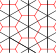
\includegraphics[width=0.46\textwidth]{dual_graph_honeycomb.pdf}%
    \hspace{0.06\textwidth}%
    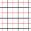
\includegraphics[width=0.46\textwidth]{dual_graph_square.pdf}%
    \caption{(left) The triangular lattice is the dual graph of the honeycomb lattice, and (right) the square lattice is the dual graph of itself.\label{fig:dualgraphs}}%
\end{figure}
\FloatBarrier

\section*{Plots for honeycomb and triangular lattices\label{sec:plots}}
\begin{figure}[h]
    \centering
    \begin{subfigure}[b]{0.49\textwidth}
        \includegraphics[width=\textwidth]{triangular_rsquared.png}
        \caption{}
        % \caption{Correlation coefficient.}
        % \label{fig:gull}
    \end{subfigure}
    \begin{subfigure}[b]{0.49\textwidth}
        \includegraphics[width=\textwidth]{triangular_giant_vs_xi.png}
        \caption{}
        % \caption{Giant component.}
        % \label{fig:tiger}
    \end{subfigure}
    \\\vspace{4mm}%
    \begin{subfigure}[b]{0.49\textwidth}
        \includegraphics[width=\textwidth]{triangular_clustersize_vs_xi.png}
        \caption{}
        % \caption{Maximum cluster size.}
        % \label{fig:mouse}
    \end{subfigure}
    \begin{subfigure}[b]{0.49\textwidth}
        \includegraphics[width=\textwidth]{triangular_qmax_vs_xi.png}
        \caption{}
        % \label{fig:cat}
    \end{subfigure}
    \caption{Results for triangular lattice. \label{fig:triangular_results}}
\end{figure}

\begin{figure}[h]
    \centering
    \begin{subfigure}[b]{0.49\textwidth}
        \includegraphics[width=\textwidth]{honeycomb_rsquared.png}
        \caption{}
        % \caption{Correlation coefficient.}
        % \label{fig:gull}
    \end{subfigure}
    \begin{subfigure}[b]{0.49\textwidth}
        \includegraphics[width=\textwidth]{honeycomb_giant_vs_xi.png}
        \caption{}
        % \caption{Giant component.}
        % \label{fig:tiger}
    \end{subfigure}
    \\\vspace{4mm}%
    \begin{subfigure}[b]{0.49\textwidth}
        \includegraphics[width=\textwidth]{honeycomb_clustersize_vs_xi.png}
        \caption{}
        % \caption{Maximum cluster size.}
        % \label{fig:mouse}
    \end{subfigure}
    \begin{subfigure}[b]{0.49\textwidth}
        \includegraphics[width=\textwidth]{honeycomb_qmax_vs_xi.png}
        \caption{}
        % \label{fig:cat}
    \end{subfigure}
    \caption{Results for honeycomb lattice. \label{fig:honeycomb_results}}
\end{figure}

% \begin{figure}%
% \centering
% \subfigure[][]{%
% % \label{fig:ex3-a}%
% \includegraphics[height=2in]{triangular_rsquared.png}}%
% % \hspace{8pt}%
% \subfigure[][]{%
% % \label{fig:ex3-b}%
% \includegraphics[height=2in]{triangular_giant_vs_xi.png}} \\
% \subfigure[][]{%
% % \label{fig:ex3-c}%
% \includegraphics[height=2in]{triangular_clustersize_vs_xi.png}}%
% % \hspace{8pt}%
% \subfigure[][]{%
% % \label{fig:ex3-d}%
% \includegraphics[height=2in]{triangular_qmax_vs_xi.png}}%
% \caption[A set of four subfigures.]{A set of four subfigures:
% \subref{fig:ex3-a} describes the first subfigure;
% \subref{fig:ex3-b} describes the second subfigure;
% \subref{fig:ex3-c} describes the third subfigure; and,
% \subref{fig:ex3-d} describes the last subfigure.}%
% \label{fig:ex3}%
% \end{figure}
\FloatBarrier

\section*{The program}
\subsection*{The main loop}
\begin{listing}[h!]
\cppfile[firstline=21, lastline=56]{../cpp_bond_percolation/src/main.cpp}%
\caption{%
    The main program. %
    \label{lst:mainloop}%
}
\end{listing}
\FloatBarrier

\subsection*{Results class}
\begin{listing}[hp!]
\cppfile[firstline=3, lastline=58]{../cpp_bond_percolation/src/results.hpp}%
\caption{%
    The \cppinline{Results} class. The \cppinline{sample} function is given in \cref{lst:samplefunction} and the \cppinline{calcResults} method is given in \cref{lst:calcresults}.%
    \label{lst:resultsclass}%
}
\end{listing}

\begin{listing}[h!]
\cppfile[firstline=3, lastline=30]{../cpp_bond_percolation/src/results.cpp}%
\caption{%
    The \cppinline{sample} method of the \cppinline{Results} class.%
    \label{lst:samplefunction}%
}
\end{listing}

\end{document}